\subsection{Hypothesis on Temporal Precision}
\label{sec:hypothesis_temporal_precision}

\begin{hypothesis}
\label{hyp:temporal_precision}
Prediction quality of queries where the prediction target is a timestamp is improved by evaluating on precision rather than rank.
\end{hypothesis}

\begin{figure}[htb]
\centering
\begin{minipage}{0.95\columnwidth}
\centering
\small
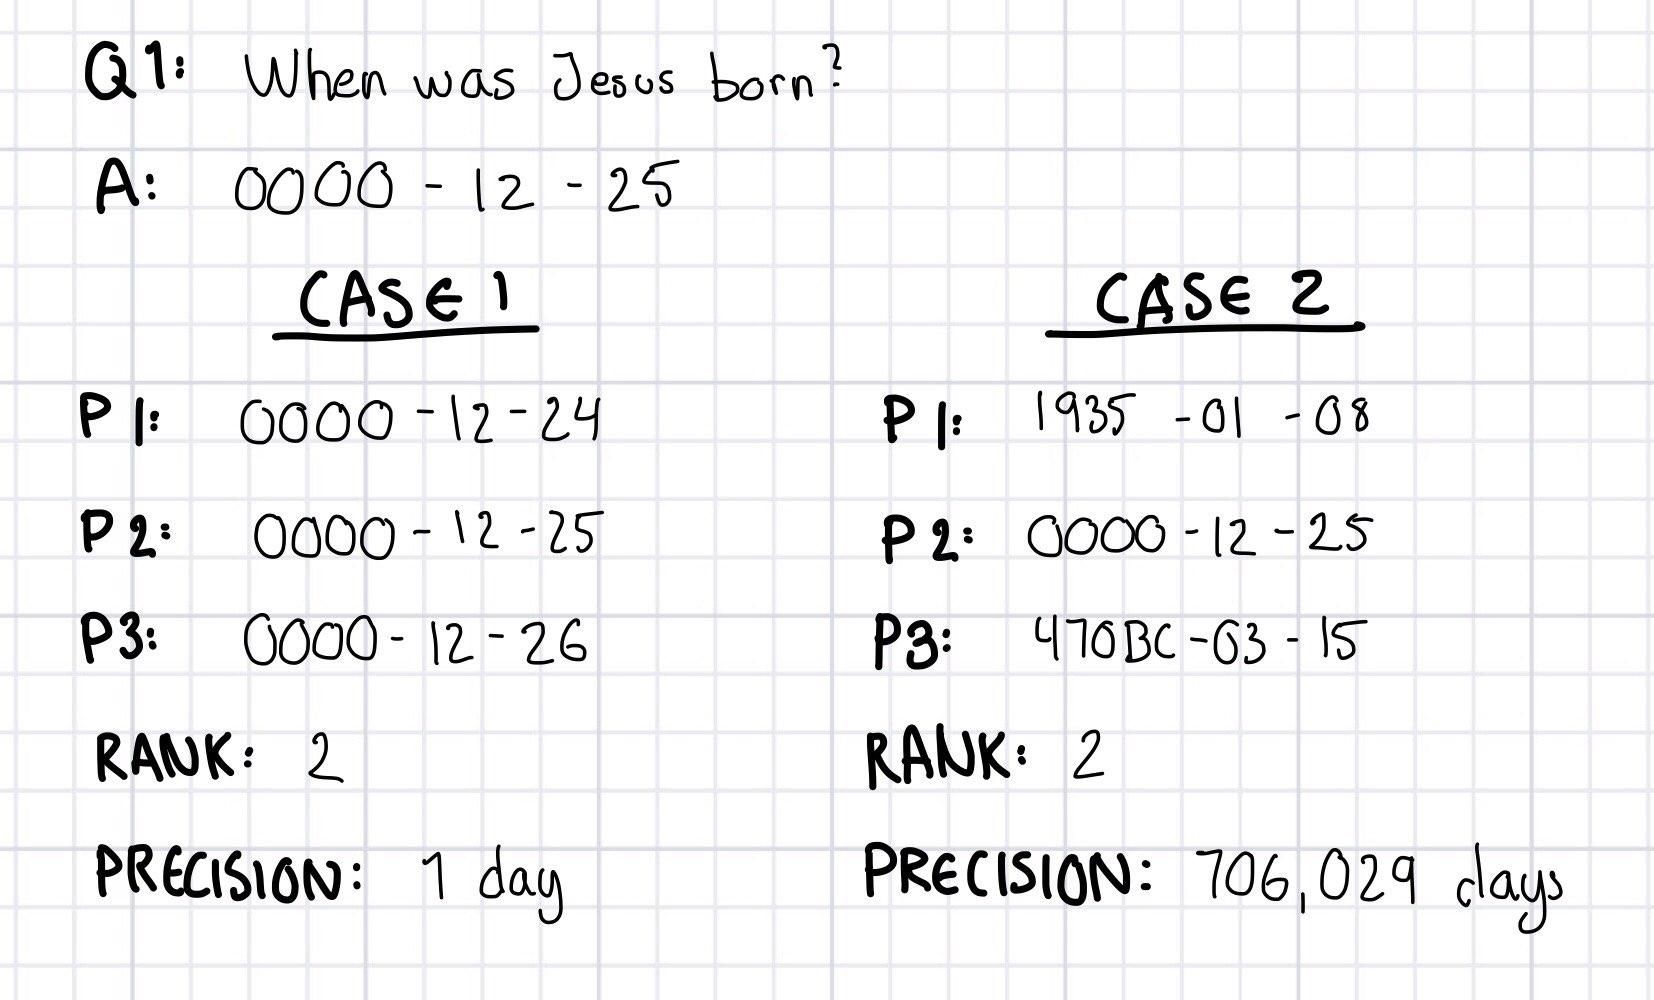
\includegraphics[scale=0.13]{content/hypotheses/figures/temporal_precision.jpg}
\caption{Illustration of \autoref{hyp:temporal_precision}. Query, Q1, has correct answer, A, and CASE1 and CASE2 are hypothetical results. For each case the top three answers by rank, the rank of the right answer and the precision of the first answer are listed.
}
\label{fig:temporal_precision}
\end{minipage}
\end{figure}

This hypothesis is inspired by prior work \cite{P9}, which showed that predictions on timestamps had considerably lower quality than predictions on other fact elements.
However, in contrast to the remaining fact elements, timestamps are a continuous rather than discrete value, and as such it is possible to measure degrees of precision.
This hypothesis is illustrated in \autoref{fig:temporal_precision}. In this example both cases rank the correct answer second, but in CASE1 the first guess is fairly close while in CASE2 it is way off. However, both cases obtain the same score.
Therefore the purpose of this hypothesis is to examine how close the  predictions on timestamps are to the correct results, instead of evaluating how far down the list of proposed results the correct one is.

To test this we need to measure the distance between predicted and correct values.
This is done both by considering the amount of correct predictions on different levels of time granularity and by calculating the distance between predicted and correct answers.